\chapter{Forschungsergebnisse: Heuristische Evaluation}
\label{app:results}\label{app:he-ergebnisse}\label{app:he-massnahmen}

Die Ergebnisse der im \sref{sec:phase1} vorgestellten Ergebnisse der Heuristischen Evaluation können online abgerufen werden:

\begin{description}
  \item[Ergebnisse] \url{https://rawgit.com/bkahlert/seqan-research/master/raw/HE-Analyse.pdf}
  \item[Maßnahmen] \url{https://rawgit.com/bkahlert/seqan-research/master/raw/HE-Massnahmen.pdf}
\end{description}

\begin{comment}
\section{Heuristische Evaluation: Ergebnisse}
\label{app:he-ergebnisse}

...


\begin{center}
  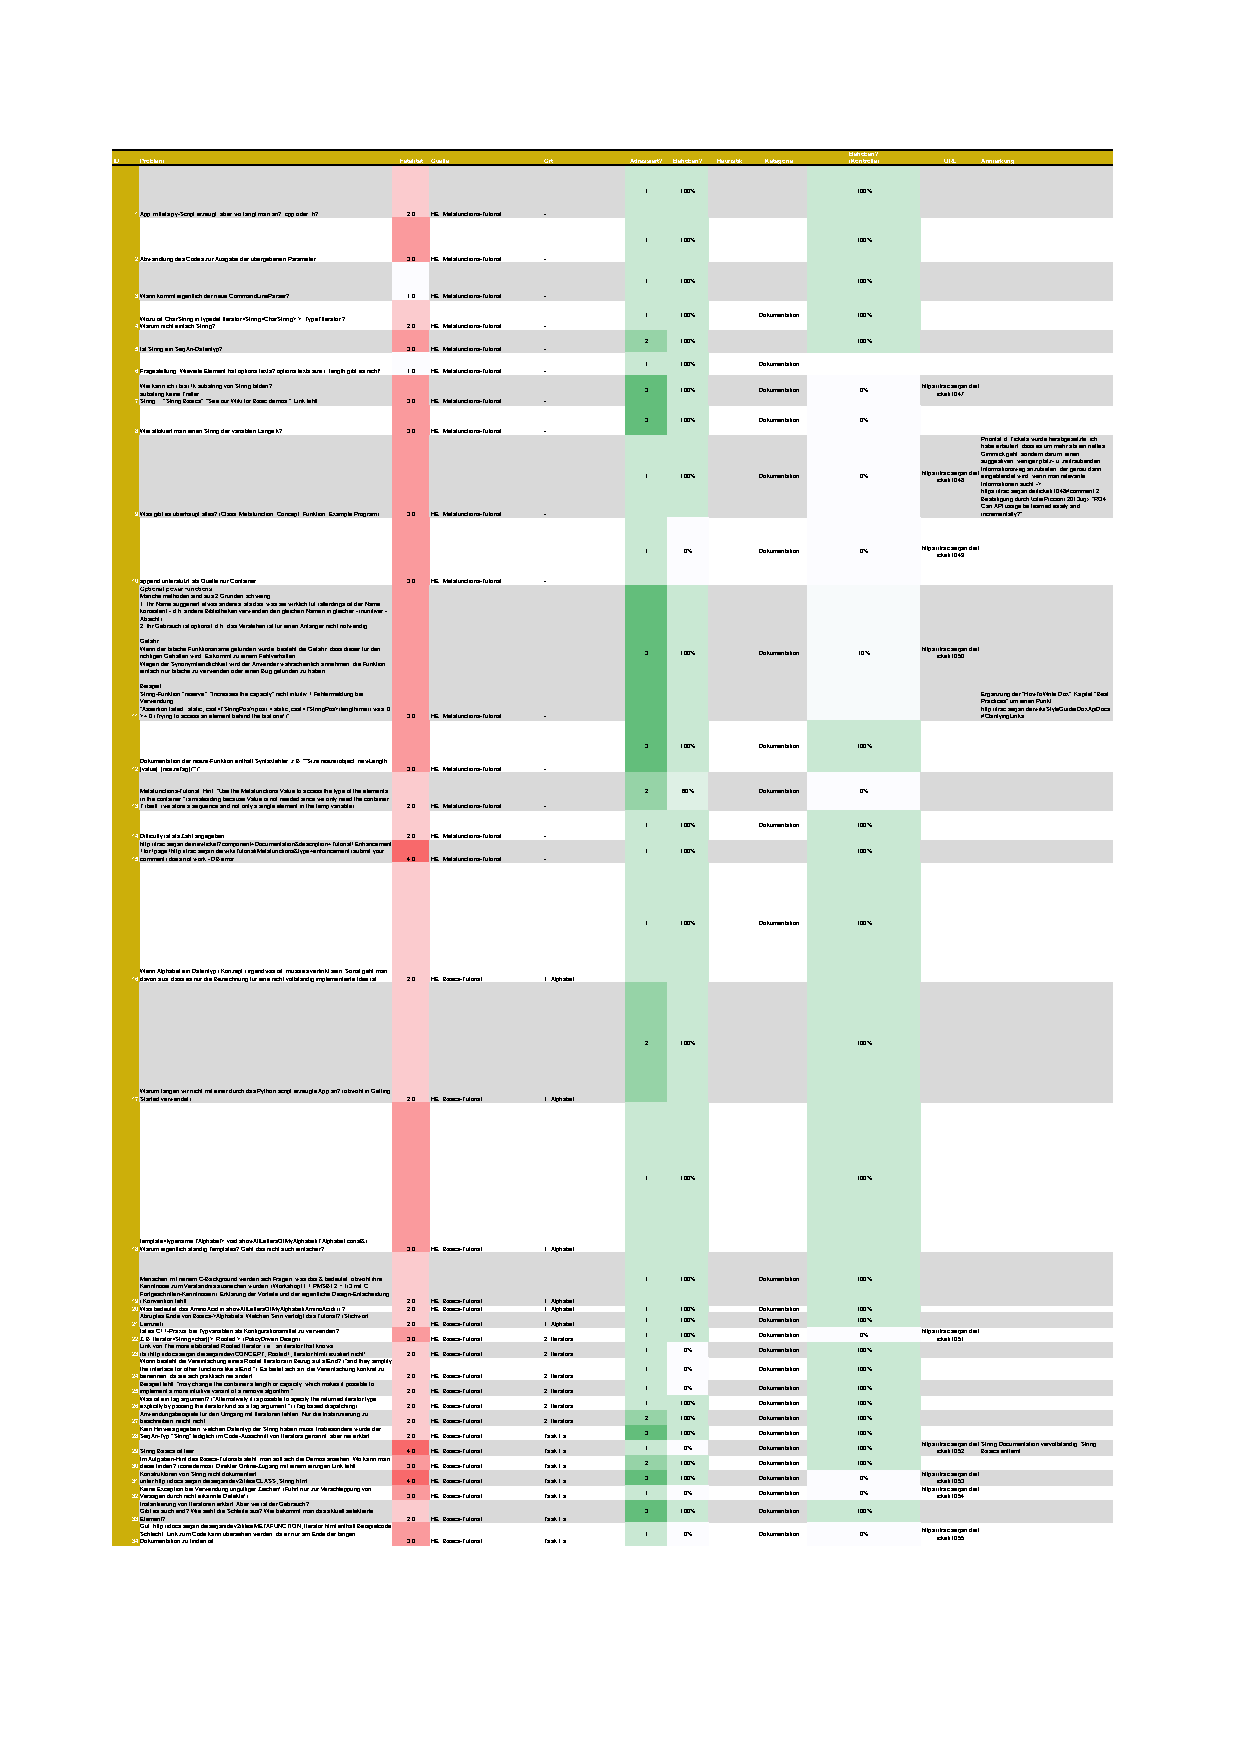
\includegraphics[page=1,width=0.85\linewidth]{Figures/HE-Analyse.pdf}
\end{center}

\begin{center}
  \includegraphics[page=2,width=0.85\linewidth]{Figures/HE-Analyse.pdf}
\end{center}

\section{Heuristische Evaluation: Maßnahmen}
\label{app:he-massnahmen}

\begin{center}
  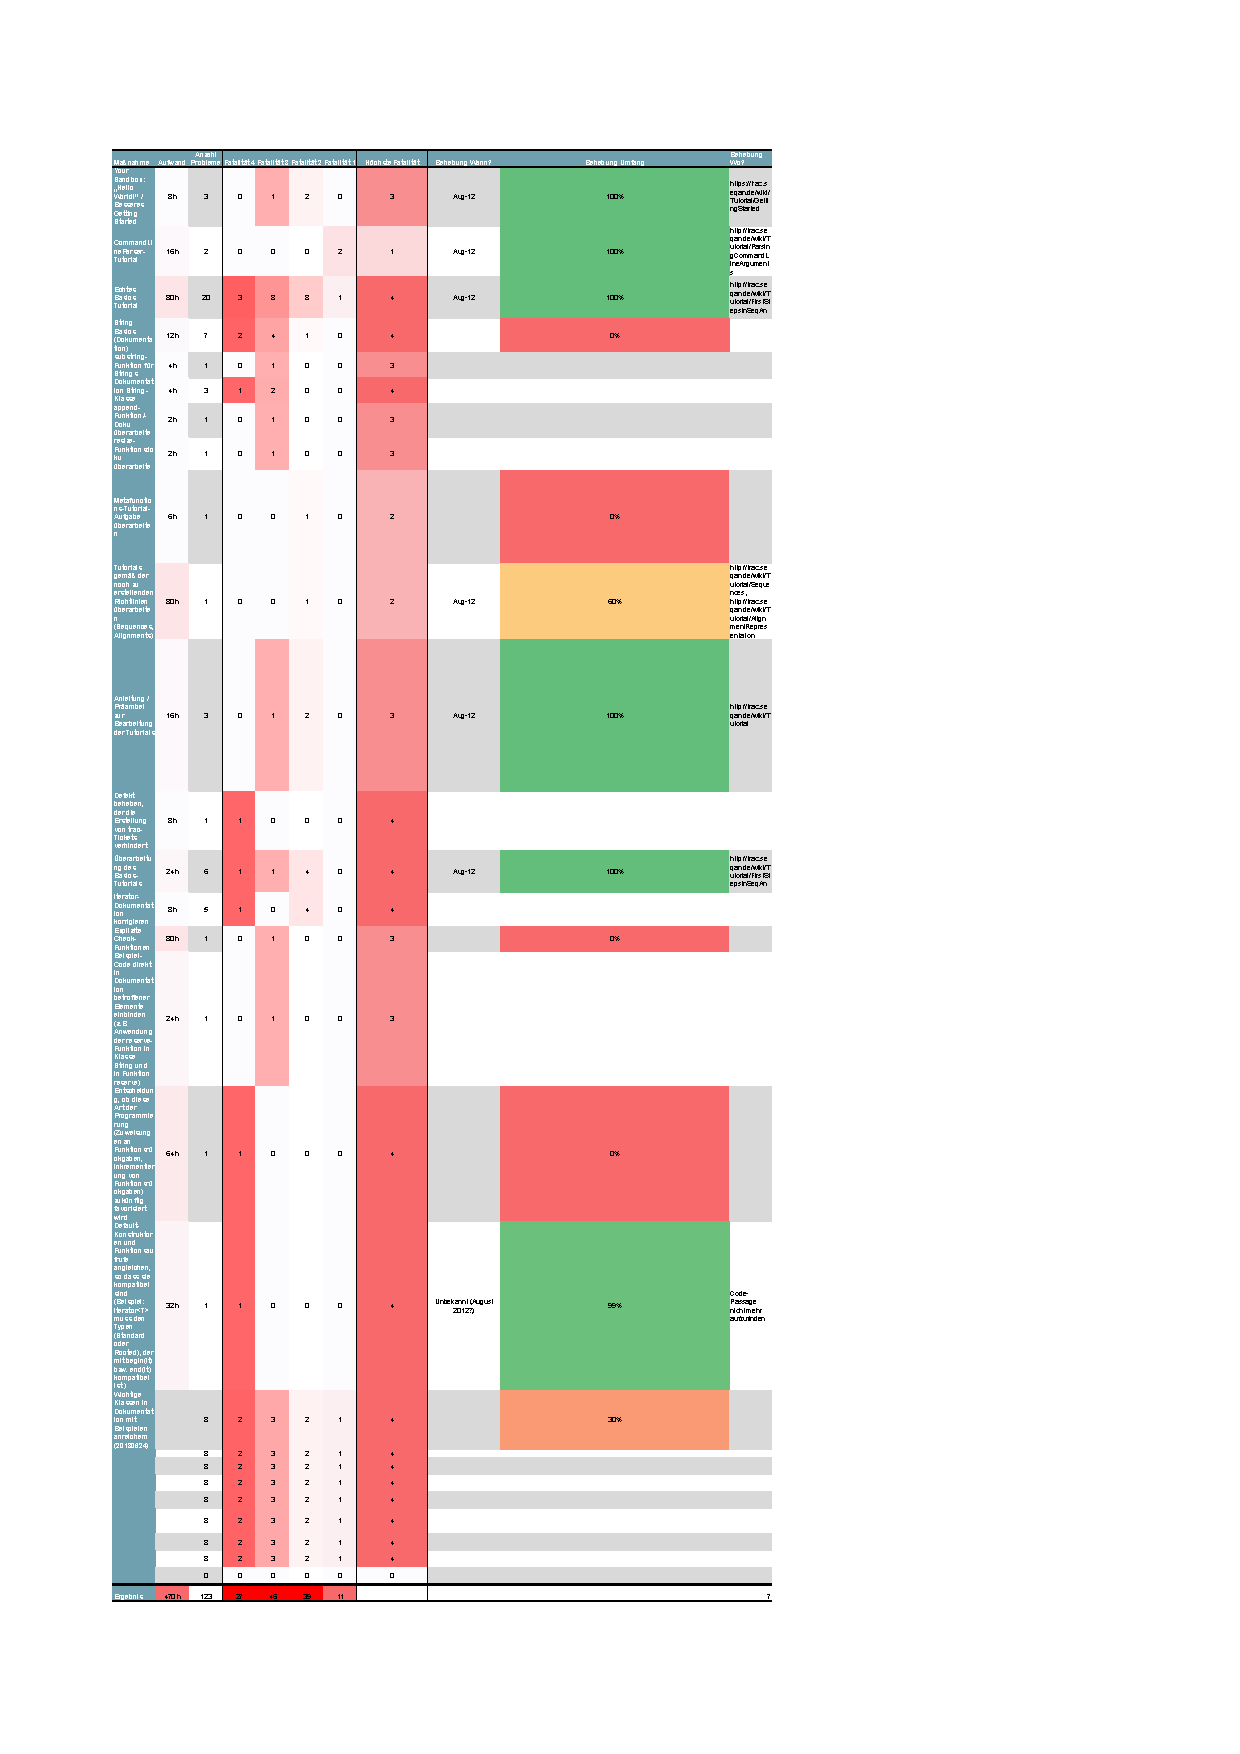
\includegraphics[page=1,width=0.85\linewidth]{Figures/HE-Massnahmen.pdf}
\end{center}
\end{comment}







\chapter{Forschungsdokumente}
\label{app:misc}



\section{Einverständniserklärung zur Datenerhebung}
\label{app:declaration-of-consent}

\begin{center}
  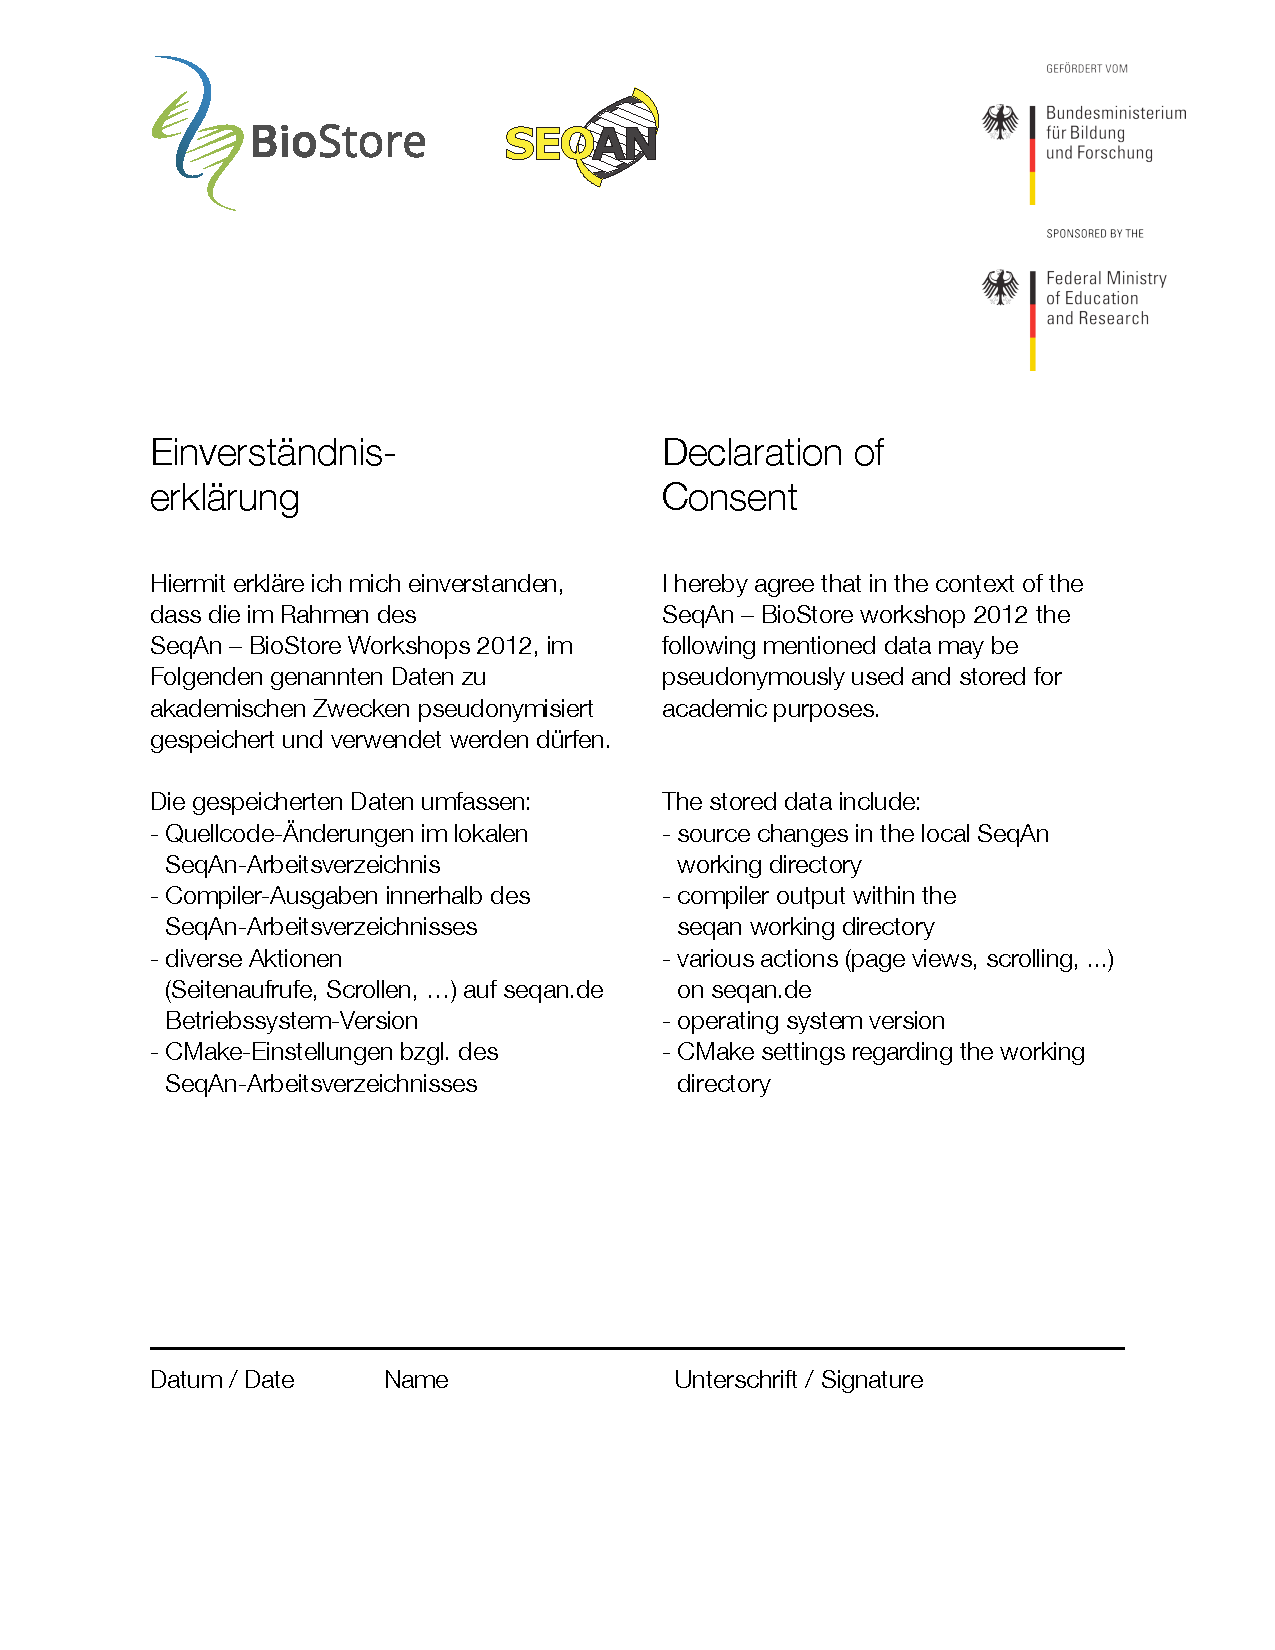
\includegraphics[width=0.85\linewidth]{Figures/declaration-of-consent.pdf}
\end{center}




\section{Online-Umfrage}
\label{app:umfrage}

\paragraph{Vorerfahrung}
\begin{itemize}
  \item What experience do you have with C, C{}\verb!++!, C{}\verb!#! and Java?
  \item Besides SeqAn, what other applications / libraries do you use?
  \item To what extend did you already work with SeqAn before the workshop?
\end{itemize}

\paragraph{Installation}
\begin{itemize}
  \item How difficult was the installation of SeqAn? (The installation includes downloading the sources, the CMake call(s) and the first run of your chosen IDE.)
  \item What did you particulary like in the installation process?
  \item What did you particularly dislike in the installation process?
\end{itemize}

\paragraph{SeqAn-Techniken}
\begin{itemize}
  \item SeqAn heavily relies on the following four C++ / SeqAn techniques (Standard Template Library (STL) and template programming, Metafunctions, Template subclassing, Global function interface).
  \item How good was your understanding and ability to correctly use each technique before the workshop?
  \item How good is your understanding and ability to correctly use each technique now that you have absolved the workshop?
\end{itemize}

\paragraph{Workshop-Tutorials} \hfill \\
\textit{(Die folgenden Fragen wurden zu jedem Tutorial gestellt, das der Proband besucht hat.)}
\begin{itemize}
  \item Did you work on this tutorial during the workshop?
  \item How would you rate your SeqAn skills concerning the tutorial topic before you have participated this workhop?
  \item Was this tutorial helpful?
  \item Could you have finished this without help by the SeqAn team?
  \item Do you think that the documentation web pages (\url{www.seqan.de}) and \url{trac.mi.fu-berlin.de/seqan}) were helpful to solve the exercises of this tutorial?
  \item While working on this tutorial: What did you particulary like? What did you particulary dislike?
\end{itemize}

\paragraph{Abschließende Fragen}
\begin{itemize}
  \item What did you particulary like about SeqAn?
  \item What did you particulary dislike about SeqAn?
  \item How would you rate the workshop altogether?
  \item How would you rate the organisation of the workshop?	
  \item How helpful was the assistance by the SeqAn staff?
  \item What do you think about the duration of the workshop?
  \item What did you expect from the workshop? Did it meet and fulfil your expectations?
  \item Will you use SeqAn in the future?
  \item What do / did you study?
  \item What is your currently highest degree?
\end{itemize}

\vfill
	 	



\section{Feedback-Zettel}
\label{app:feedback}

\setlength{\fboxsep}{0pt}%
\setlength{\fboxrule}{0.3pt}%

\subsection*{Kickoff-Feedback-Zettel}
\begin{center}
  \fbox{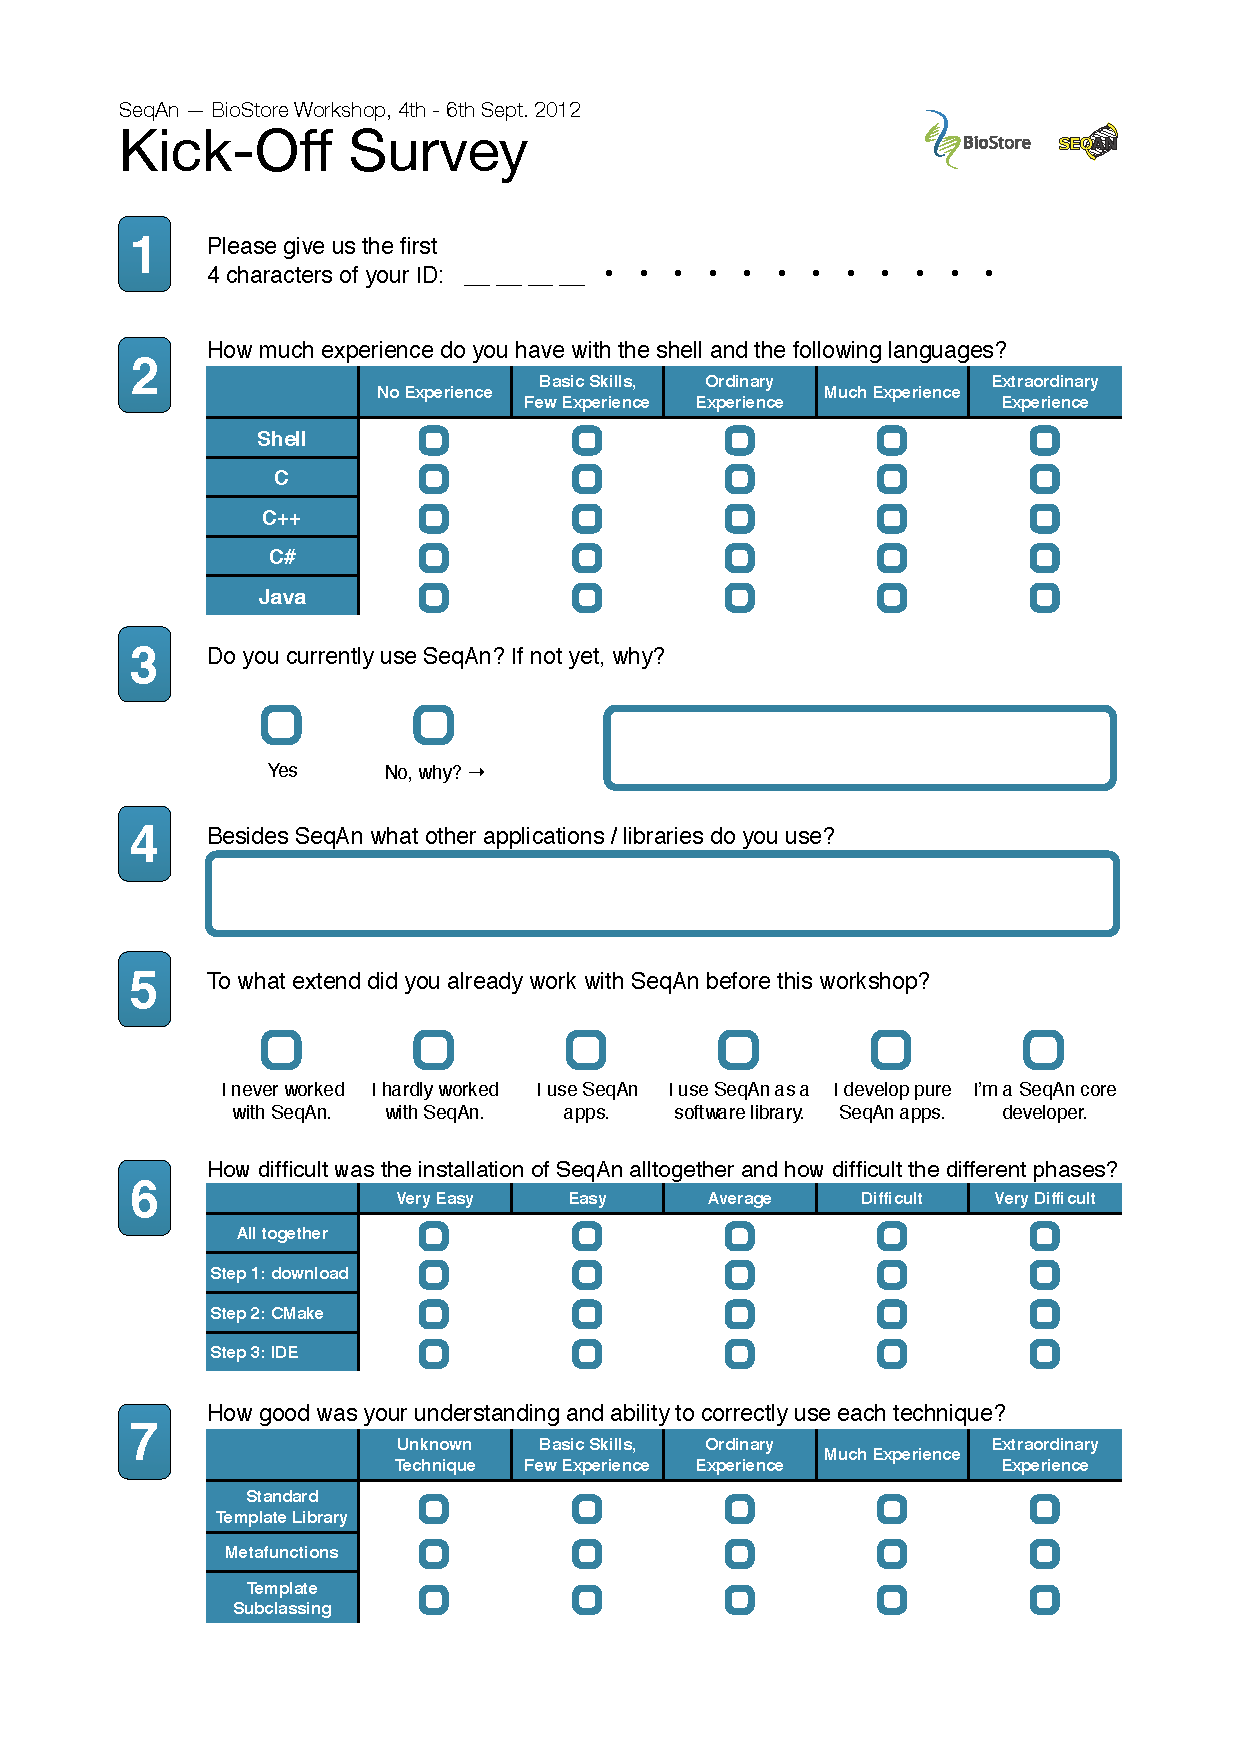
\includegraphics[width=0.85\linewidth]{Figures/feedback-kickoff-workshop12.pdf}}
\end{center}

\subsection*{Tutorial-Feedback-Zettel}
\begin{center}
  \fbox{\includegraphics[width=0.95\linewidth,page=3]{Figures/feedback-tutorial-workshop12.pdf}}
\end{center}

\subsection*{Abschluss-Feedback-Zettel}
\begin{center}
  \fbox{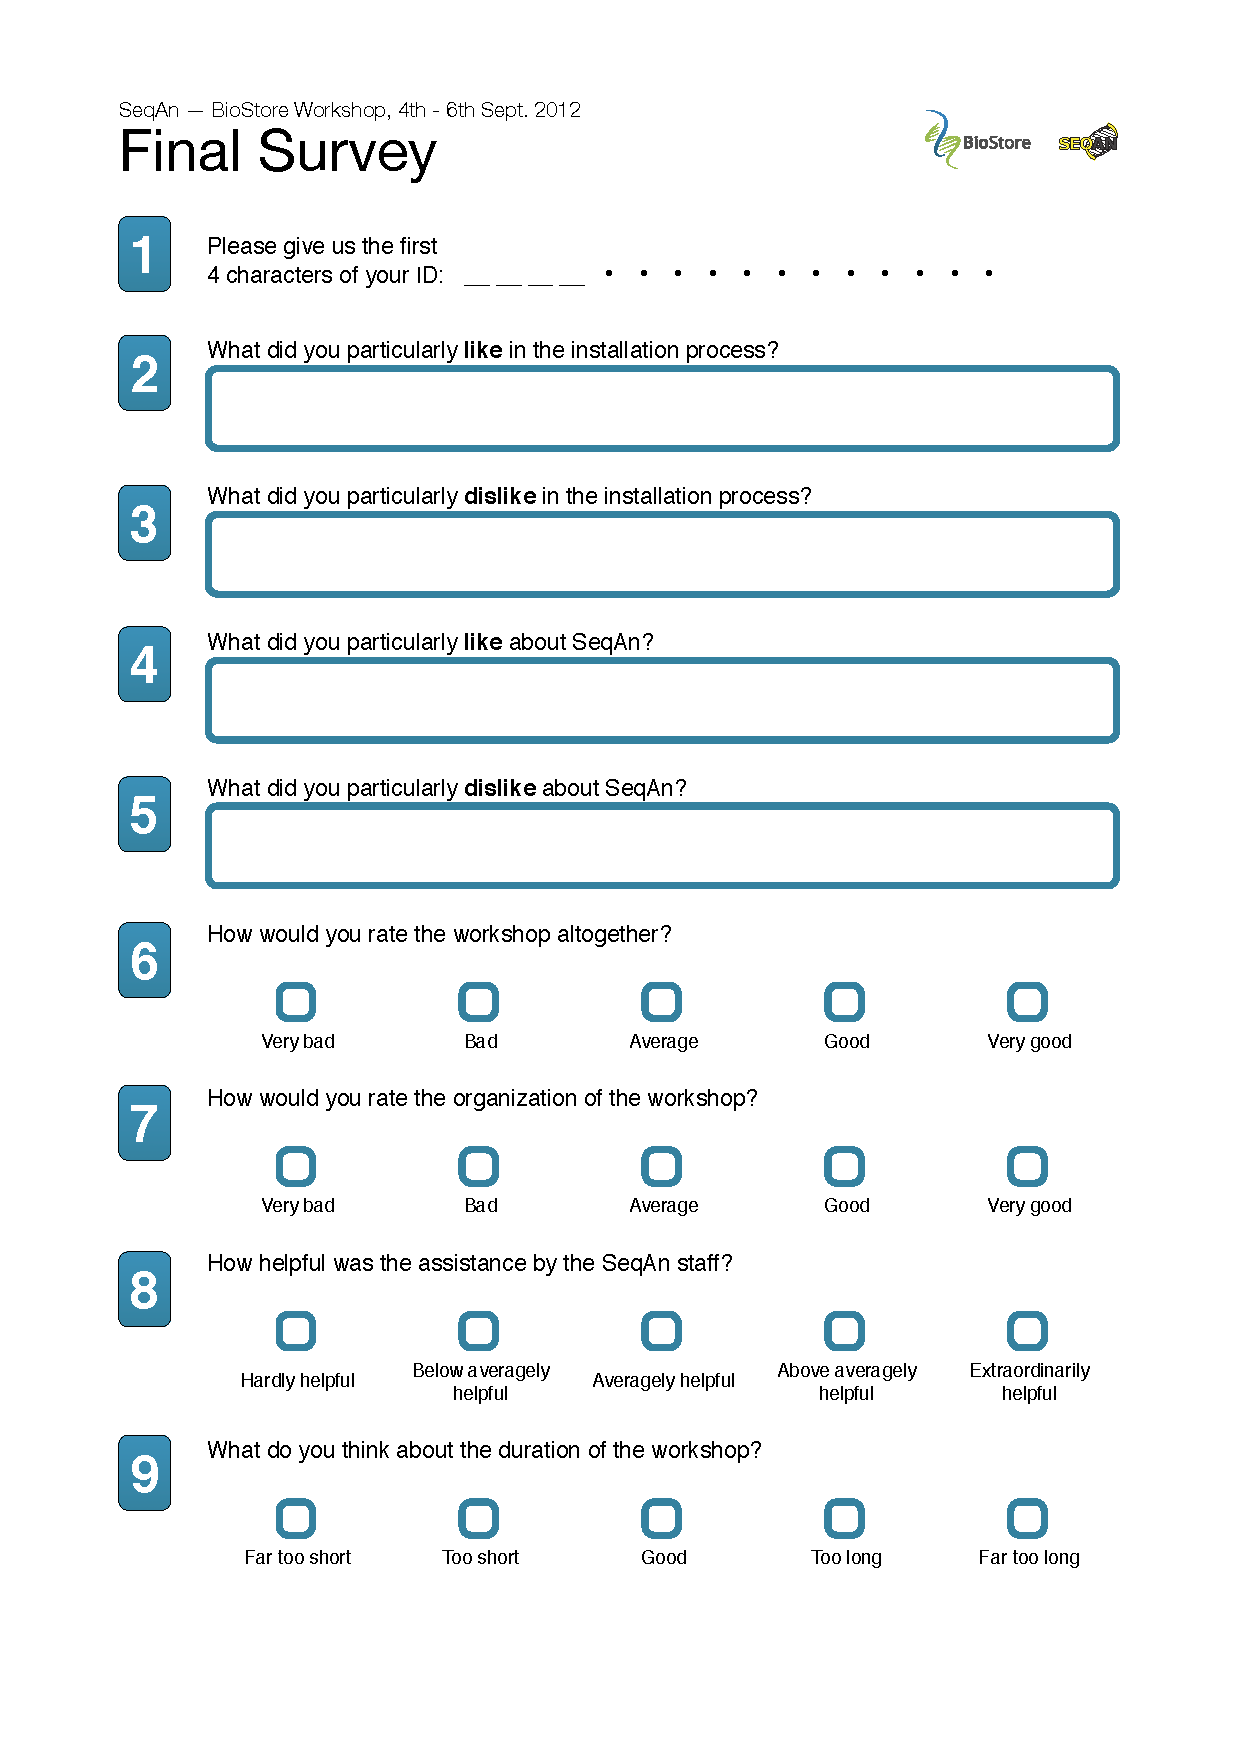
\includegraphics[width=0.95\linewidth,page=1]{Figures/feedback-final-workshop12.pdf}}
\end{center}
\begin{center}
  \fbox{\includegraphics[width=0.95\linewidth,page=2]{Figures/feedback-final-workshop12.pdf}}
\end{center}


\vfill


\section{Cognitive-Dimensions-Fragebogen}
\label{app:cd-fragebogen}

Der näher im \sref{sec:cdf-usage} vorgestellte Cognitive-Dimensions-Fragebogen kann online abgerufen werden:

\begin{description}
  \item[Deutsch] \url{https://rawgit.com/bkahlert/seqan-research/master/raw/workshop13/cd-fragebogen-de.pdf}
  \item[Englisch] \url{https://rawgit.com/bkahlert/seqan-research/master/raw/workshop13/cd-fragebogen-en.pdf}
\end{description}

Die Fragen aus Teil 3 des Fragebogens beziehen sich auf jeweils eine \gls{cd} und waren für die Befragten nicht sichtbar. Sie konnten lediglich die Fragen selbst sehen. Die erfragten CDs des Fragebogens, die, wenn nicht anders angegeben, von \cite{Anonymous:9HSMlhmF} stammen, lauten:

\begin{enumerate}
\itemsep1pt\parskip0pt\parsep0pt
  \item Anpassungsfreundlichkeit \textit{API Viscosity}
  \item Arbeitsschrittgröße / Codedichte (\textit{Work-Step Unit})\footnote{Diese \gls{cd} stammt von \cite{Anonymous:9HSMlhmF} und ist eine Spezialisierung der \gls{cd} \textit{Diffuseness} von \cite{161956}.}
  \item Arbeitsgedächtnisanforderungen (\textit{Hard Mental Operations})\footnote{Dabei handelt es sich um eine \gls{cd} von \cite{161956}. Von \cite{Anonymous:9HSMlhmF} wird sie als \textit{Working Framework} bezeichnet.}
  \item Fehleranfälligkeit (\textit{Error Proneness})\footnote{Dabei handelt es sich um eine Dimension nach \cite{161956}.}
  \item Fachbezogenheit (\textit{Domain Correspondence})
  \item Rollenerkennbarkeit (\textit{Role Expressiveness})
  \item Fortschreitende Evaluation (\textit{Progressive Evaluation})
  \item Vorläufigkeit (\textit{Provisionality})\footnote{Dabei handelt es sich um eine Dimension nach \cite{161956}.}
  \item Verfrühter Entscheidungszwang (\textit{Premature Commitment})
  \item Konsistenz (\textit{Consistency})
  \item Abstraktionsebenen (\textit{Abstraction Level})
  \item Lernweise (\textit{Learning Style})
\end{enumerate}

%nicht enthalten
%\item[Durchdringbarkeit (\textit{Penetrability})] In welchem Umfang wird der API-Anwender unterstützt, die Komponenten der API zu explorieren, zu analysieren zu verstehen? Wie gelangt der API-Anwender an diese Informationen?
%\item[API-Anpassungnotwendigkeit (\textit{API Elaboration})] In welchem Umfang muss die API angepasst werden, um die Bedürfnissen eines API-Anwenders zu erfüllen?


\begin{comment}
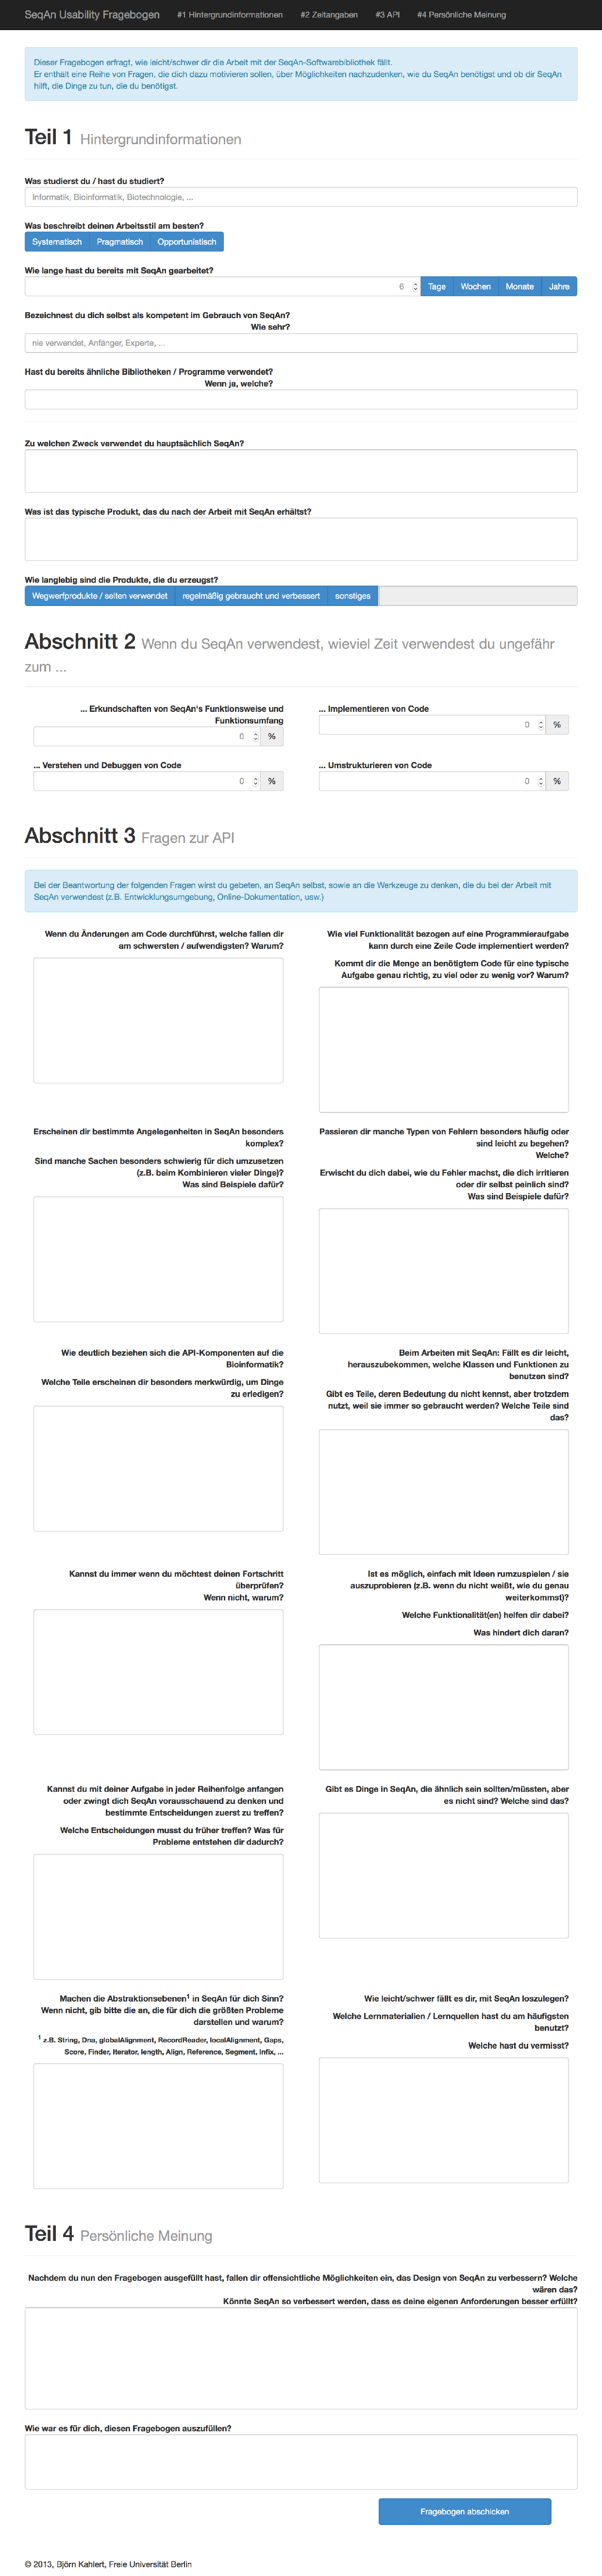
\includepdf[fitpaper=true,addtolist={1,figure,Fragebogen zu kognitiven Dimensionen \textit{(Deutsch)},fig:cd-fragebogen-de}]{Figures/cd-fragebogen-de.pdf}

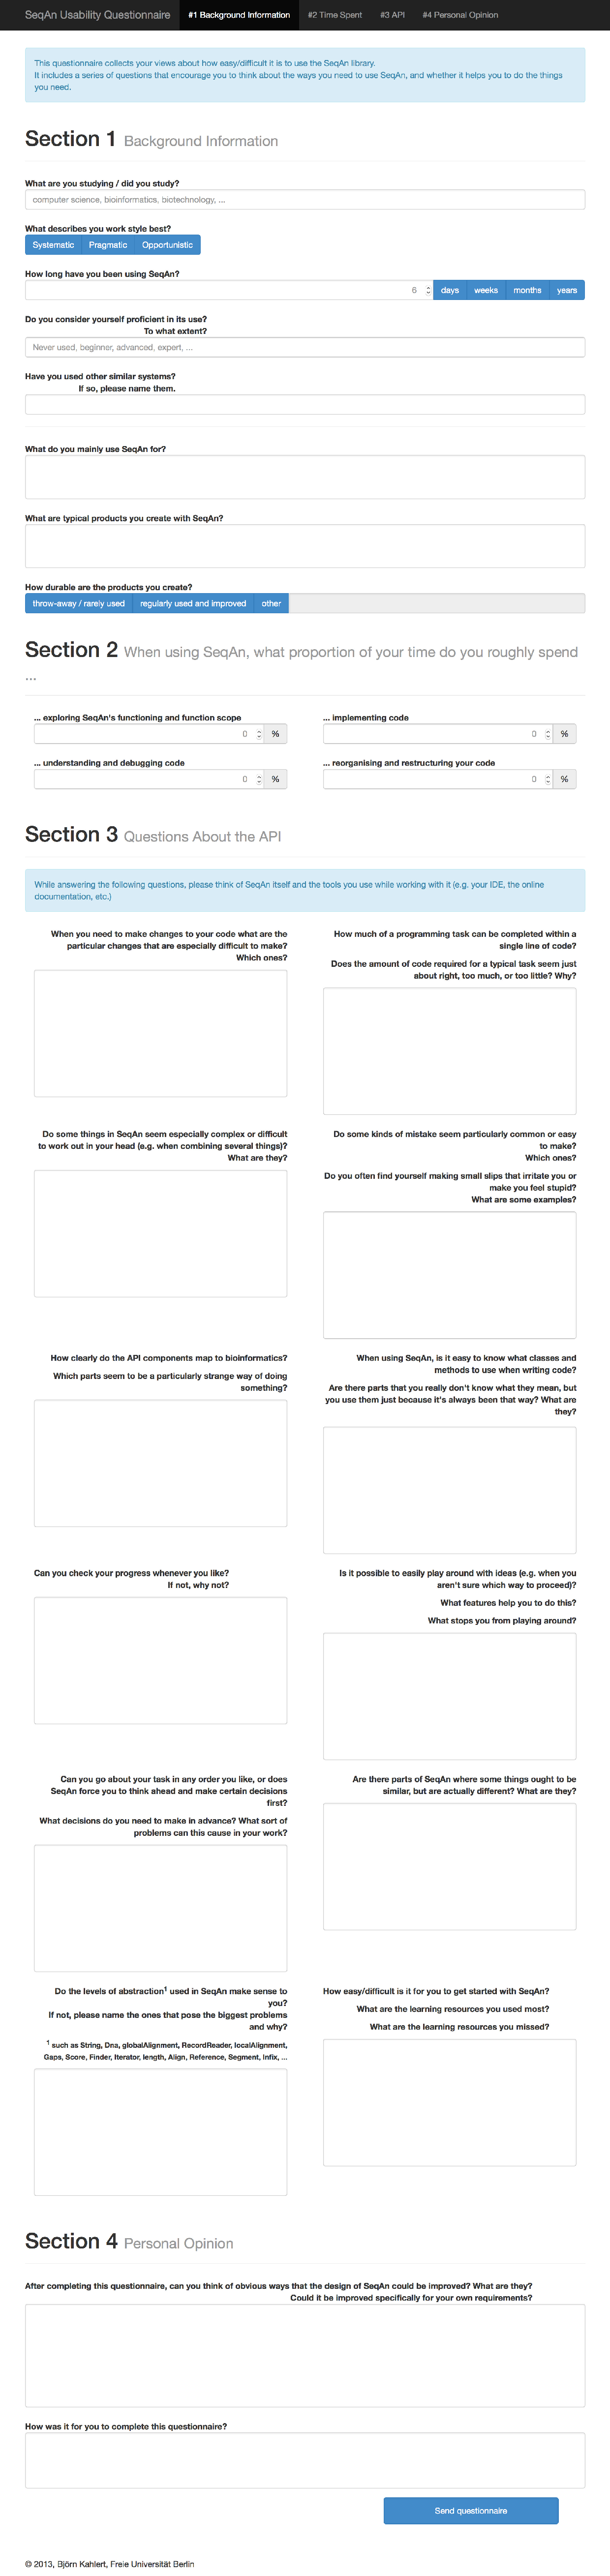
\includepdf[fitpaper=true,addtolist={1,figure,Fragebogen zu kognitiven Dimensionen \textit{(Englisch)},fig:cd-fragebogen-en}]{Figures/cd-fragebogen-en.pdf}

\begin{figure}
  \centering
  \begin{subfigure}[b]{0.30\linewidth}
    \centering
    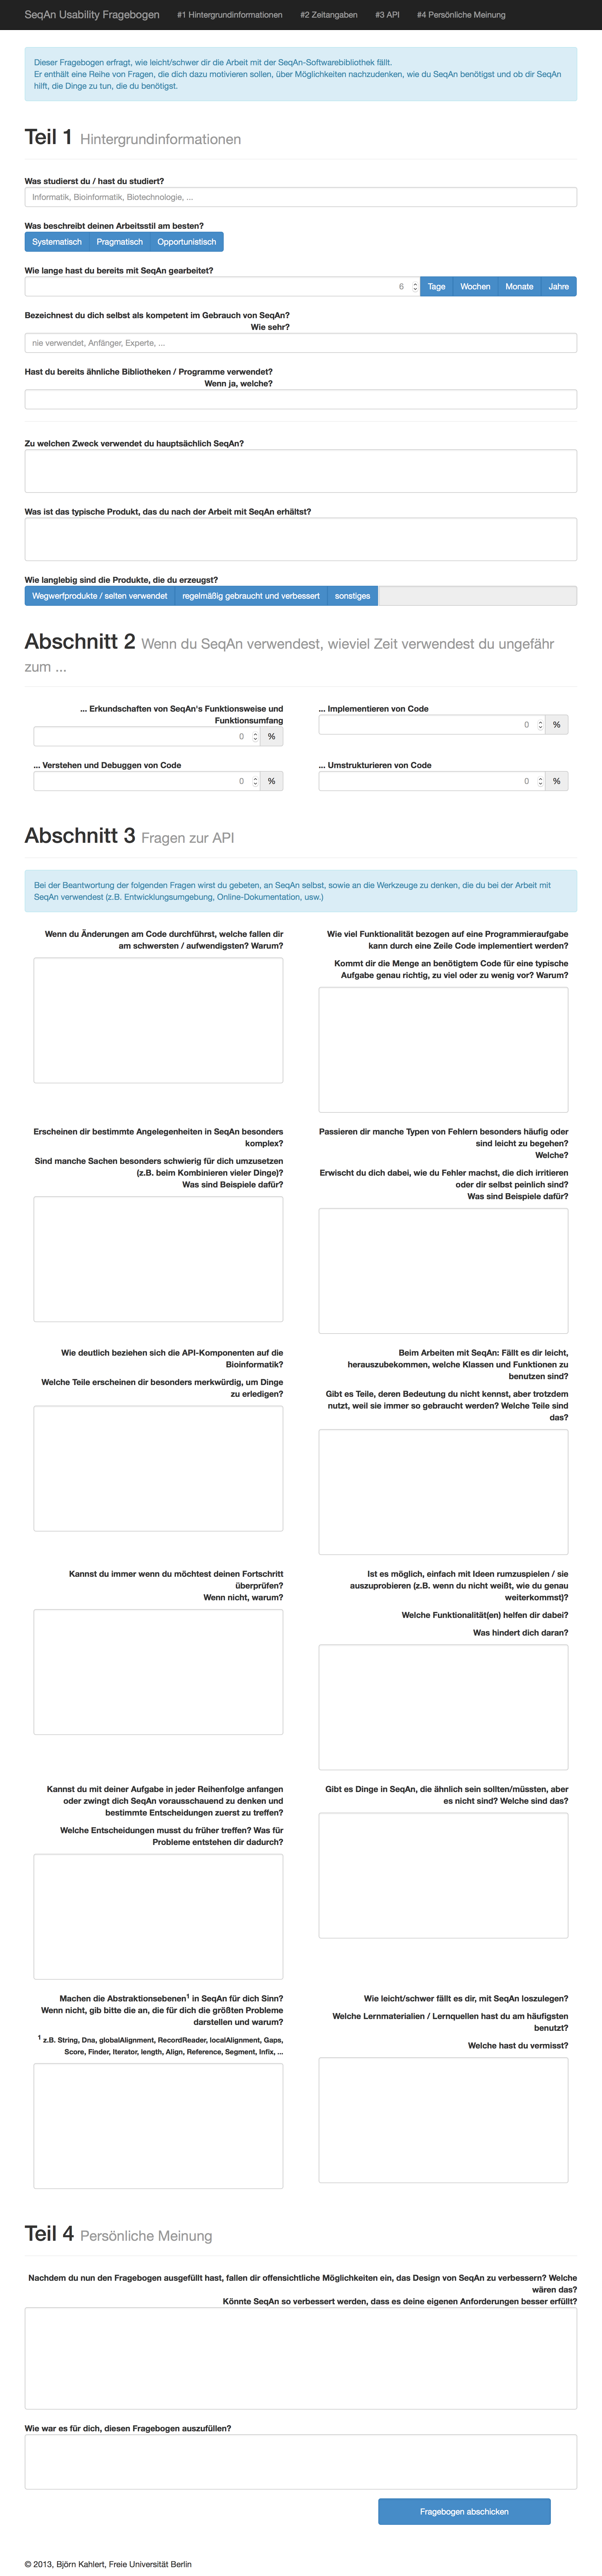
\includegraphics[width=\linewidth]{Figures/cd-fragebogen-de.png}
    \caption{Deutsch}
    \label{fig:cd-fragebogen-de}
  \end{subfigure}%
  \hfill%
  \begin{subfigure}[b]{0.30\linewidth}
    \centering
    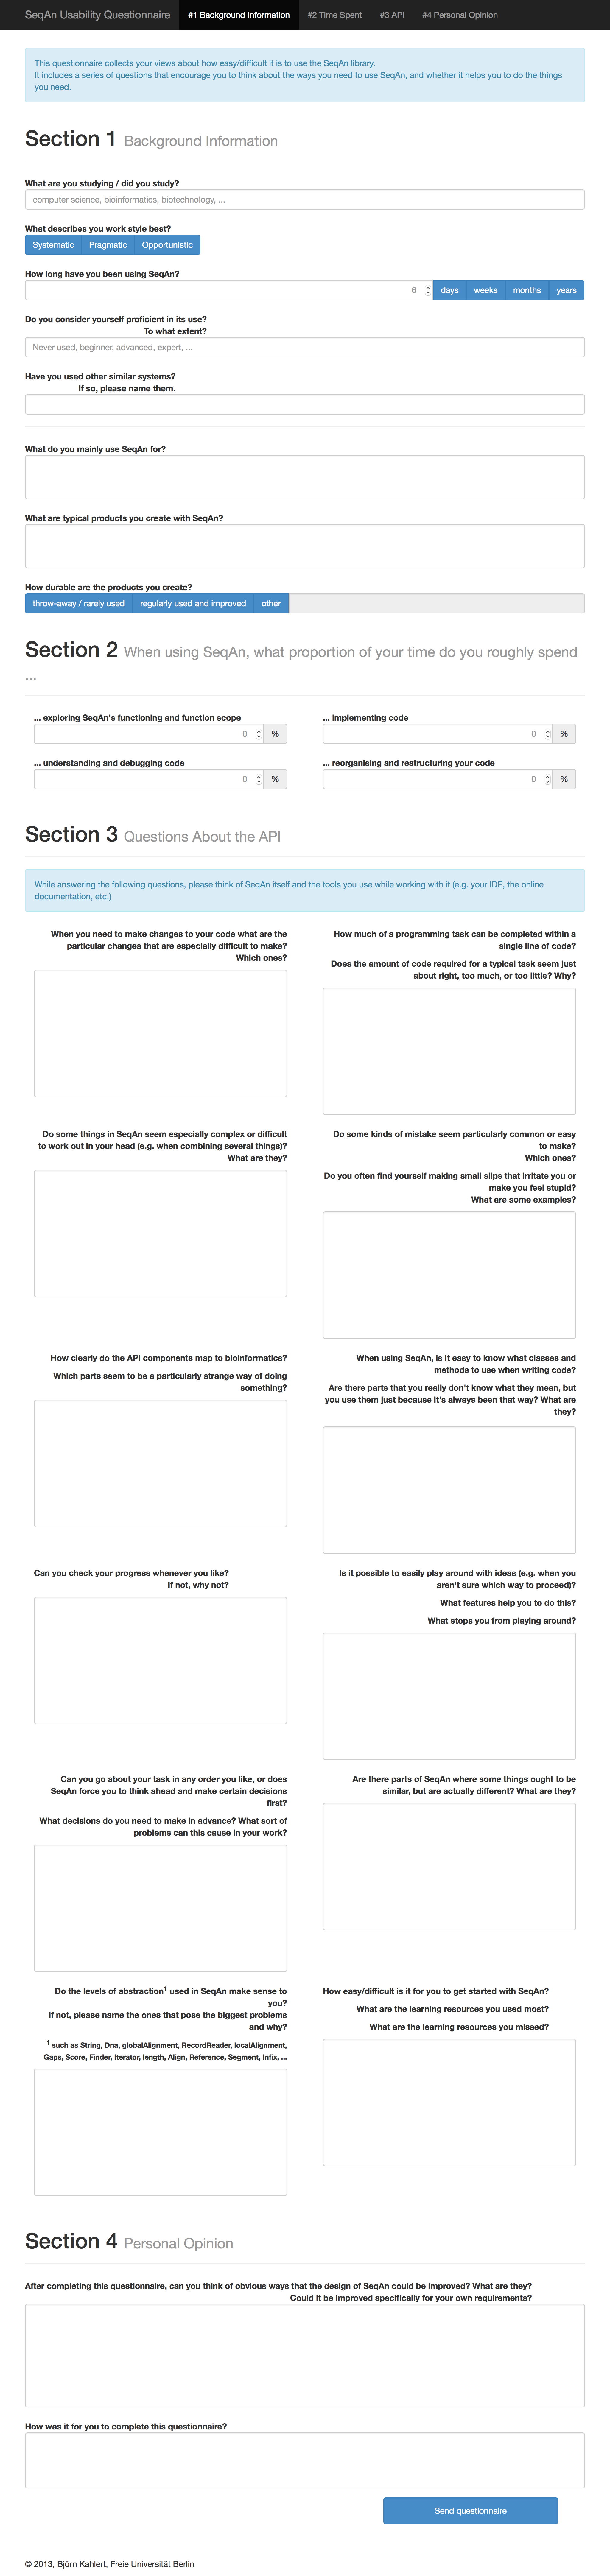
\includegraphics[width=\linewidth]{Figures/cd-fragebogen-en.png}
    \caption{Englisch}
    \label{fig:cd-fragebogen-de}
  \end{subfigure}%
  \caption{Online-Fragebogen zu kognitiven Dimensionen}%
  \label{fig:cd-fragebogen}%
\end{figure}
\end{comment}